\newpage
\section{Part A}
\label{sec:sec_a}
The dataset was generated using a simulated circuit in LTSpice. The diode using test is a model of the \textit{1N4148} and the current limiting resistor has a value of 15 $\Omega$. 

\begin{figure}[htpb]
	\centering
	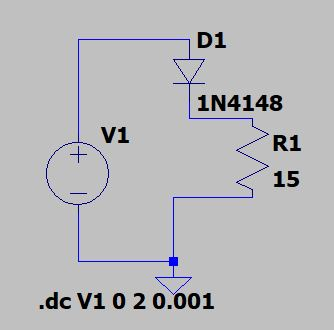
\includegraphics{figures/lt_spice_diagram.JPG}
	\caption{LTSpice Schematic}
	\label{fig:lt_schematic}
\end{figure}

The voltage source \textit{V1} was simulated to sweep from 0V to 2V DC. At each step measurements were taken for \textit{V}$_{d}$ and \textit{I}$_{d}$, the voltage across the diode and current respectively. Figure~\ref{fig:lt_current} plots the diode current as a function of voltage. As can be seen there is a clear exponential relationship between the two values.

\begin{figure}[!htpb]
	\centering
	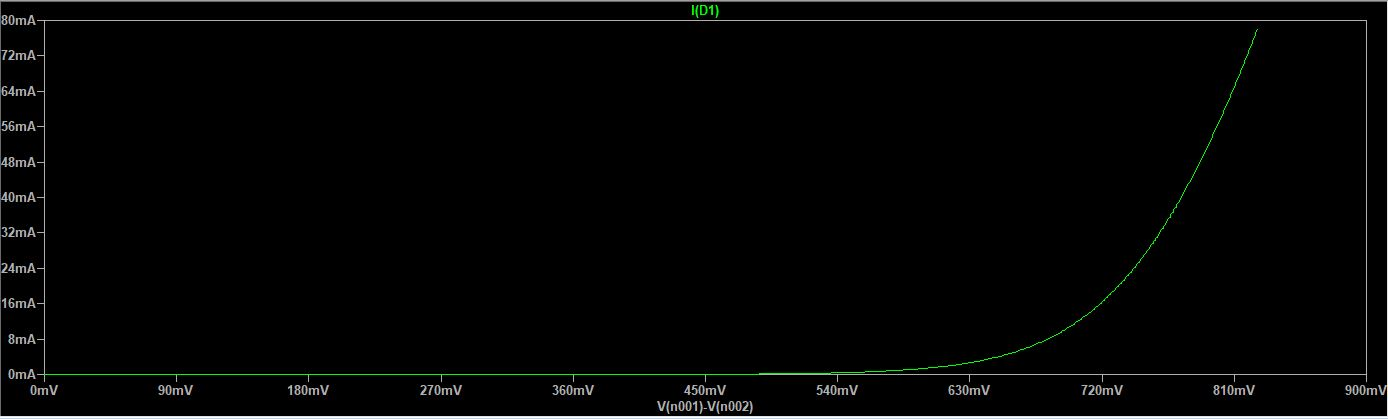
\includegraphics[width=\columnwidth]{figures/lt_spice_plot.JPG}
	\caption{\textit{I}$_{d}$ vs \textit{V}$_{d}$}
	\label{fig:lt_current}
\end{figure}

Because the dataset is being generated synthetically errors representing those of a typical multimeter are introduced. The synthetic error follows the error metrics for the \textit{Agilent U1272A} presented in the project guide lines. Using the synthetically noisy voltage measurement \textit{I}$_{d}$ was computed as $I_{d} = V_{d}/15$, which produces a noisy current measurement as opposed to the pristine simulated value.
\newpage
\LST{part\_a}